\chapter{METHODOLOGY}
\section{Methodology}

For the study of research methods, or, more formally, ‘a contextual framework' for research of this project, spiral model was chosen among all others as it enables gradual releases and refinement of a product through each phase of the spiral as well as the ability to build prototypes at each phase. Spiral model is one of the most important Software Development Life Cycle models, which provides support for Risk Handling. It has four phases: Planning, Design, Construct and Evaluation. A software project repeatedly passes through these phases in iterations (called Spirals in this model) as shown in the figure below. The Radius of the spiral at any point represents the expenses (cost) of the project so far, and the angular dimension represents the progress made so far in the current phase. In each phase of the Spiral Model, the features of the product dated and analyzed, and the risks at that point in time are identified and are resolved through prototyping.
\vspace{0.2cm}
\begin{figure}[h]
    \centering
    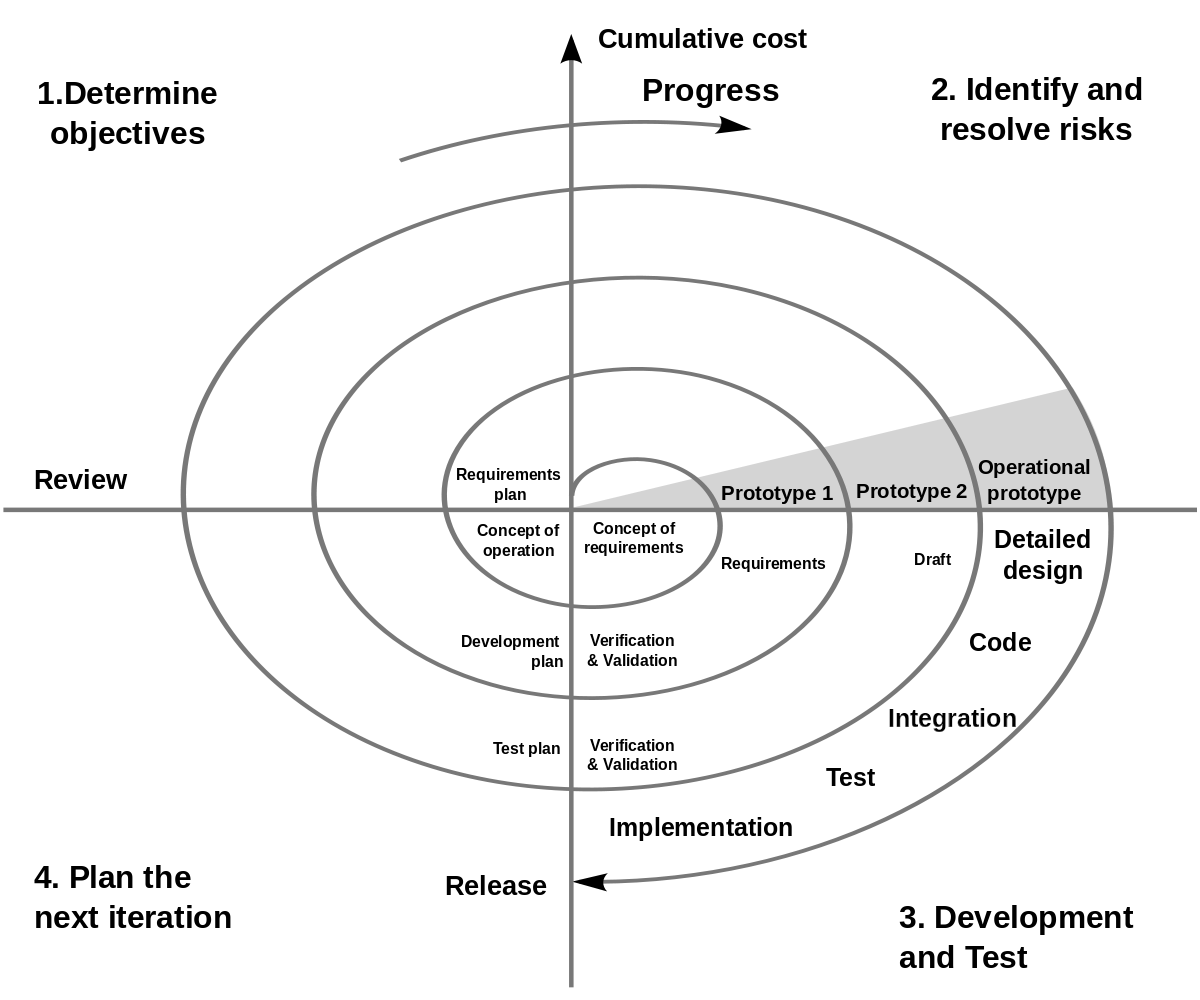
\includegraphics[width=120mm]{images/spiral.png}
    \caption{Spiral Model of Software Development}
    \label{fig:Spiral Model}
\end{figure}
\vspace{1cm}
\begin{itemize}
    \item \textbf{Planning Phase}\\
Requirements are gathered from the customers and the objectives are
identified, elaborated, and analyzed at the start of every phase. Then
alternative solutions possible for the phase are proposed in this quadrant.
     \item \textbf{Risk Analysis Phase}\\
     During the second quadrant, all the possible solutions are evaluated to
select the best possible solution. Then the risks associated with that
solution are identified and the risks are resolved using the best possible
strategy. At the end of this quadrant, the Prototype is built for the best
possible solution.
     
      \item \textbf{Development and Testing Phase}\\
      During the third quadrant, the identified features are developed and
verified through testing. At the end of the third quadrant, the next version
of the software is available.
       \item \textbf{Evaluation and Planning next Phase}\\
       In the fourth quadrant, the Customers evaluate the so far developed version
of the software. In the end, if the Customers are satisfied with the software,
then, it is released, else, planning for the next phase is started.
       
\end{itemize}
